\section{Results and Discussion}

\subsection{Analysis of Model Performance}

Results on the AI-ELT dataset were much better compared to the ART-Net dataset (see Tables \ref{fig:modelresults} and \ref{fig:artresults}). Due to the more distinct edges, more straightforward scenes with less background motion, and lack of occlusion, smoke, glare, and other major visual artefacts, we suspect this makes it easier for the models to detect the tools. The AI-ELT dataset also has a higher resolution, which may have contributed to the better results. The anchor-free YOLOv8-X model was the most accurate, achieving a mAP$_{50}$ of 99.5\% and a mAP$_{50:95}$ of 85.6\% on the test set with an inference time of 21.7ms, approximately 46 frames-per-second (FPS), demonstrating its effectiveness in real-time surgical tool detection. The most efficient model was YOLOv8-N, achieving a mAP$_{50}$ of 99.5\% and a mAP$_{50:95}$ of 83.3\% at 1.8ms/555 FPS (with only 3 million parameters and 6.2MB weights - ~20x less than YOLOv8-X at 136.7MB). SIMO vastly underperformed compared to the original ART-Net results. As part of an ablation study, we included detection after segmentation using a fully connected layer (FCN), which produced excellent results on the ART-Net dataset, notwithstanding even higher inference times, but could not be performed for the AI-ELT dataset due to lack of segmentation maps. EfficientDet performed similarly to YOLOv10-X on the ART-Net dataset yet could not match this on AI-ELT. DETR continuously improved even with the 300-generation limit, benefiting the most from more data and extended training. 

Generally, YOLO architectures N and X performed marginally better than others. This is surprising as one would expect greater performance with larger networks. We expect the smaller architecture was forced to generalise better with fewer parameters. Direct model comparisons show that there was not necessarily a correlation between higher accuracy using a more complex architecture, though logically it does result in higher inference times. It is possible that smaller networks could generalise better and faster than larger models, which may have slightly overfitted (still, with YOLOv8-N, we notice poorer generalisation in difficult examples). With more data samples and extended training, we expect the larger models to inevitably outperform the smaller models consistently. The best model, YOLOv8-X, trained the longest of any YOLO models, contributing to this claim. Though YOLOv8 and YOLOv10 vary in many other properties, which could be investigated further, we expect that anchor-free methods outperformed anchor-box methods. We suspect RetinaNet was an exception to this due to anchor-box optimisation even in the base model. The non-anchor-based methods, EfficientDet and DETR, likely require more data and longer fine-tuned training for better results. YOLOv8's unique data augmentation, appropriate loss function, and anchor-free architecture give it excellent performance. Overall, the methods used across all models were the same, and thus, the results were reliable even though some were not as accurate as expected. 

% DIAGRAMS
\footnotesize
\begin{table*}[htbp]
    \centering
    \caption{Laparoscopic Tool Detection Results on the AI-ELT Dataset.}
    \vspace*{-3mm}
    \label{fig:modelresults}
    \begin{tabular}{|c|c|c|c|c|c|c|c|c|c|c|c|c|}
    \hline
    \multicolumn{2}{|c|}{\textbf{Model}} & \multicolumn{3}{c|}{\textbf{mAP$_{50}$}} & \multicolumn{3}{c|}{\textbf{mAP$_{50:95}$}} & \multicolumn{2}{c|}{\textbf{Inference}} & \multicolumn{3}{c|}{\textbf{Training}} \\
    \hline
    \textbf{Name} & \textbf{Size} $^a$ & \textbf{Tool} & \textbf{Tooltip} & \textbf{Both} & \textbf{Tool} & \textbf{Tooltip} & \textbf{Both} & \textbf{Time (ms)} & \textbf{FPS} & \textbf{Epochs} & \textbf{TT} $^b$ & \textbf{T/E} $^c$ \\ 
    \hline
    \multicolumn{13}{|c|}{\textbf{Anchor-Based}} \\
    \hline
    YOLOv10-X & 31.7 (\textbf{688}) & 98.9 & 99.1 & 99.0 & 93.5 & 68.4 & 81.0 & 19.3 & 52 & 19 & 7.8 & 0.41 \\ 
    YOLOv10-L & 25.8 (628) & 98.9 & 98.3 & 98.6 & 89.4 & 67.0 & 78.2 & 13.0 & 77 & 15 & 3.5 & 0.23 \\ 
    YOLOv10-B & 20.5 (518) & 98.7 & 99.0 & 98.9 & 92.2 & 69.3 & 80.8 & 10.3 & 97 & 14 & 2.2 & 0.16 \\ 
    YOLOv10-M & 16.5 (498) & 98.2 & 98.7 & 98.5 & 90.5 & 69.1 & 79.8 & 8.0 & 125 & 14 & 1.6 & 0.11 \\ 
    YOLOv10-S & 8.1 (402) & 99.3 & 99.2 & 99.3 & 92.7 & 69.1 & 80.9 & 3.9 & 256 & 16 & 1.8 & 0.11 \\ 
    YOLOv10-N & 2.7 (385) & 99.1 & 99.1 & 99.1 & 93.5 & 69.9 & 81.7 & 2.2 & 465 & 19 & 1.9 & 0.10 \\ 
    RetinaNet & 36.4 (195) & \textbf{99.9} & 98.4 & 99.2 & 89.1 & 65.3 & 77.2 & 5.1 & 196 & 99 & 25.7 & 0.26 \\ 
    RetinaNet-Opt $^d$ & 36.4 (195) & \textbf{99.9} & 98.5 & 99.2 & 88.3 & 66.7 & 77.5 & 5.2 & 192 & 25 & 2.2 & 0.09 \\ 
    EfficientDet & 6.6 (552) & N/A & N/A & 48.5 & N/A & N/A & 33.7 & 4.0 & 250 & 162 & 4.8 & 0.03 \\ 
    \hline
    \multicolumn{13}{|c|}{\textbf{Anchor-Free}} \\
    \hline
    \rowcolor{yellow} YOLOv8-X $^e$ & \textbf{68.2} (385) & 99.5 & \textbf{99.4} & \textbf{99.5} & \textbf{96.6} & \textbf{74.6} & \textbf{85.6} & 21.7 & 46 & 84 & 18.6 & 0.22 \\ 
    YOLOv8-L & 43.6 (365) & 99.5 & \textbf{99.4} & \textbf{99.5} & 95.2 & 73.0 & 84.1 & 12.8 & 78 & 36 & 1.6 & 0.05 \\ 
    YOLOv8-M & 25.9 (295) & 99.5 & \textbf{99.4} & \textbf{99.5} & 94.5 & 73.7 & 84.1 & 8.0 & 125 & 29 & 1.7 & 0.06 \\ 
    YOLOv8-S & 11.1 (225) & 99.5 & \textbf{99.4} & \textbf{99.5} & 96.0 & 73.9 & 85.0 & 3.4 & 294 & 66 & 1.0 & \textbf{0.02} \\ 
    \rowcolor{pink} YOLOv8-N $^f$ & 3.0 (225) & 99.5 & \textbf{99.4} & \textbf{99.5} & 94.5 & 72.0 & 83.3 & \textbf{1.8} & \textbf{556} & 41 & \textbf{0.8} & \textbf{0.02} \\ 
    SIMO-Resnet $^g$  & 23.5 (231) & 15.6 & 12.5 & 14.1 & 13.4 & 10.9 & 12.2 & 350.0 & 3 & 16 & 1.3 & 0.08 \\ 
    SIMO-VGG $^h$  & 14.7 (98) & 19.3 & 16.2 & 17.8 & 15.7 & 13.0 & 14.4 & 1280.0 & 1 & 26 & 13.0 & 0.50 \\ 
    DETR & 41.5 (318) & 49.5 & 49.0 & 49.3 & 46.3 & 32.3 & 39.3 & 35.9 & 28 & \textbf{294} & 16.2 & 0.06 \\
    \hline
\end{tabular}
% go to next line
\newline
\scriptsize{$^a$ Trainable parameters in millions and layers in brackets. $^b$ Training Time (in hours). $^c$ Time per epoch (in hours). $^d$ Anchor-based with anchor box optimisation. $^e$ The overall best-performing model. $^f$ The overall best-performing model on the ART-Net dataset. $^g$ The augmented Single Input Multiple Output (SIMO) ART-Net model using an alternative ResNet50 backbone. $^h$ Using the standard VGG-16 backbone.}
\vspace{-2.5mm}
\end{table*}

\footnotesize
\begin{table}[htbp]
\centering
\caption{Object Detection Results on the ART-Net Dataset $^a$.}
\vspace*{-3mm}
\label{fig:artresults}
\begin{tabular}{|c|c|c|c|c|c|c|}
\hline
\multicolumn{1}{|c|}{} & \multicolumn{3}{c|}{\textbf{mAP$_{50}$}} & \multicolumn{3}{c|}{\textbf{mAP$_{50:95}$}} \\
\hline
\textbf{Model Name} & \textbf{Tool} & \textbf{Tooltip} & \textbf{Both} & \textbf{Tool} & \textbf{Tooltip} & \textbf{Both} \\ 
\hline
\multicolumn{7}{|c|}{\textbf{Anchor-based}} \\
\hline
YOLOv10-X & 75.3 & 43.1 & 59.2 & 55.4 & 20.8 & 38.1 \\
% YOLOv10-L & 57.3 & 29.0 & 43.2 & 35.0 & 12.2 & 23.6 \\
% YOLOv10-B & 69.0 & 43.0 & 56.0 & 46.7 & 21.6 & 34.2 \\
% YOLOv10-M & 69.6 & 26.9 & 48.3 & 46.4 & 11.0 & 28.7 \\
% YOLOv10-S & 68.4 & 46.1 & 57.3 & 49.3 & 20.2 & 34.8 \\
YOLOv10-N & 75.3 & 53.6 & 64.5 & 57.3 & 28.6 & 43.0 \\
RetinaNet & 86.9 & 66.5 & 76.7 & 57.1 & 41.4 & 49.3 \\
RetinaNet-Opt & 90.1 & 69.4 & 79.8 & 60.0 & \textbf{43.3} & 51.7 \\
EfficientDet & N/A & N/A & 57.0 & N/A & N/A & 38.7 \\
\hline
\multicolumn{7}{|c|}{\textbf{Anchor-free}} \\
\hline
\rowcolor{pink} YOLOv8-X $^b$ & 88.9 & 67.5 & 78.2 & 70.1 & 32.8 & 51.5 \\
% YOLOv8-L & 90.4 & 61.9 & 76.2 & 70.0 & 28.6 & 49.3 \\
% YOLOv8-M & 89.8 & 65.2 & 77.5 & 66.0 & 33.0 & 49.5 \\
% YOLOv8-S & \textbf{93.8} & 76.5 & 85.2 & 75.2 & 37.1 & 56.2 \\
\rowcolor{yellow} YOLOv8-N $^c$ & \textbf{92.9} & \textbf{80.4} & \textbf{86.7} & \textbf{76.2} & \textbf{43.3} & \textbf{59.8} \\
SIMO-Resnet & 17.4 & 10.1 & 13.8 & 16.9 & 15.1 & 16.0 \\
SIMO-VGG & 19.1 & 12.1 & 15.6 & 18.8 & 11.7 & 15.2 \\
DETR & 23.7 & 13.3 & 18.5 & 13.1 & 13.3 & 13.2 \\
\hline
\end{tabular}
\newline
\scriptsize{$^a$ Selected models only. Excluded training information. Due to the smaller image sizes, inference times were almost identical, though slightly faster than on AI-ELT. $^b$ The overall best-performing model on the AI-ELT dataset. $^c$ The overall best-performing model.}
\vspace{-4mm}
% $^b$ The overall best-performing model on AI-ELT. $^c$ The overall best-performing model.
\end{table}

\normalsize

\subsection{Qualitative Results}

\begin{figure}[htbp]
    \centering
    \vspace*{-3mm}
    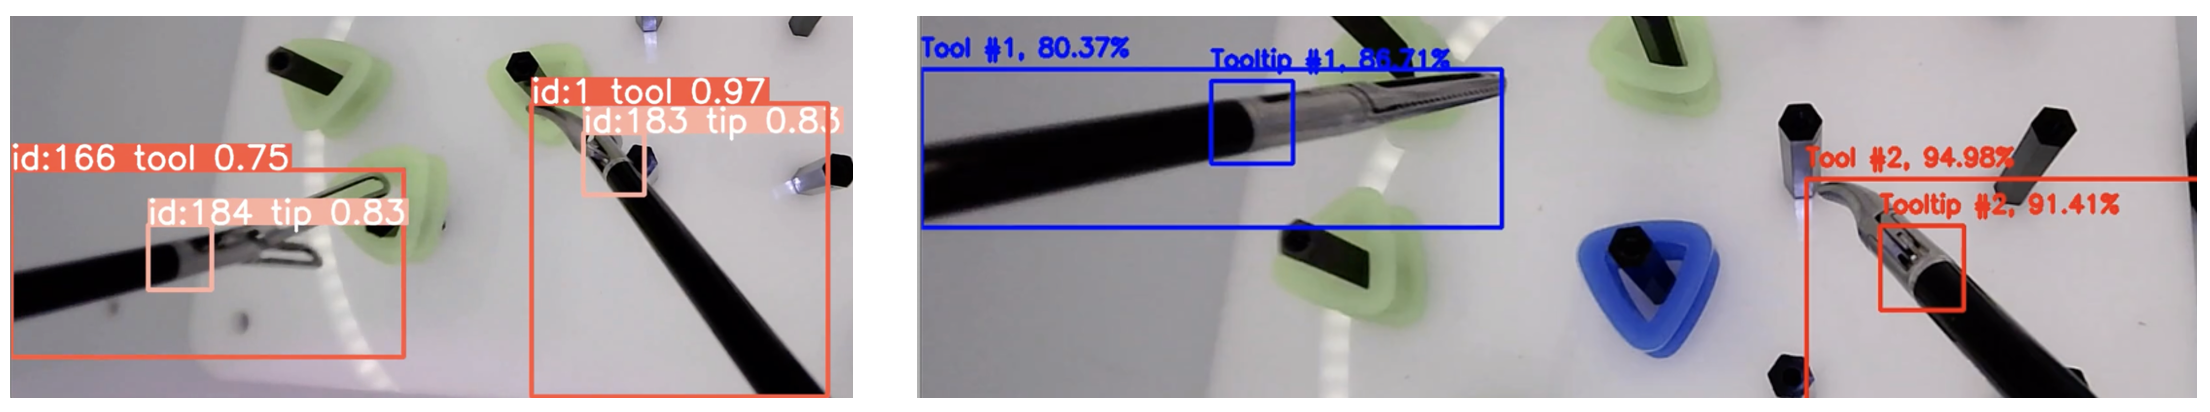
\includegraphics[width=1\linewidth]{test5_results.png}
    \vspace*{-7.5mm}
    \caption{Tool Detection and Tracking Results.}
    \vspace*{-2.5mm}
    \label{fig:test5_results}
    \Description{Tool Detection and Tracking Results using the YOLOv8-X model with YOLO tracking (left), in-house tracking (right) and original annotations (top).}
\end{figure}

Figure \ref{fig:test5_results} shows detection and tracking results using the YOLOv8-X model. ByteTrack (\textit{left}) and BoT-SORT often assign a new identification tag to a tooltip when re-identified, even when the tip was entirely in the frame, resulting in large identification values and very poor tracking accuracy. Though we do not have actual tracking data to compare with, the preliminary results suggest that our proposed tracking algorithm (\textit{right}) achieves 100\% accuracy for already detected left tool and tip (blue) and right tool and tip (right). The different YOLO architectures suggested increasing parameters, increased tracking stability and more accurate localisation (not to be confused with accuracy, which also seemed to increase). However, the RetinaNet was generally more consistent and stable, though it sometimes introduced a third tool during tool overlap. Notably, the given YOLO configurations displayed swift convergence, with a usable model after a handful of epochs. We can also conclude that using anchor boxes seemed to reduce YOLOv10 accuracy given its similar architecture to YOLOv8, yet slightly worse performance when tools appear with partial occlusion, overlap, or abnormal aspect ratios. RetinaNet had the best performance in these instances, suggesting the anchor-box optimisation (even without our additional optimisation) assisted in its performance under challenging examples. SIMO seemed to approximate the position of the tool in the image but was not precise with bounding box locations - it likely did not learn enough about the features of the data. Experimenting with segmentation on ART-Net resulted in excellent performance after much longer training, though this was not possible on AI-ELT due to a lack of data.

% \subsection{Model Usability}

% The AI-ELT dataset differs significantly from in-vivo datasets, leading to better results due to more straightforward scenes and higher data quality. This is observed when comparing our investigation on the ART-Net dataset and against SOTA models on other datasets. However, the models' usability is focused on an in-vitro context, excluding the most well-known surgical and laparoscopic datasets. YOLO models showed rapid convergence to usable solutions and are lightweight (6.2MB weights for the smallest YOLOv8-N and 136.7MB for the largest YOLOv8-X) and run in real-time but may require testing on less capable hardware.
% The AI-ELT dataset differs significantly from in-vivo datasets, leading to better results with simple models due to more straightforward scenes and higher data quality than other datasets. However, the models' usability is focused on an in-vitro context, excluding many laparoscopic datasets. The real-time YOLO models are lightweight (6.2MB weights for N and 136.7MB for X) but may require testing on less capable hardware.

%Deploying a model on a server and using an Application Programming Interface (API) to interact by sending requests over the internet from even a mobile phone may be even more feasible in cases where establishing an internet connection would be cheaper than new hardware, especially if there are many surgical training bootcamp locations. In its current stage, the models' intended users would be researchers and developers. There would be no interaction with input data handling unless there is the intention to fine-tune a model for new datasets, such as with proprietary machines at a specific hospital.

\subsection{Limitations}

The AI-ELT dataset differs significantly from in-vivo datasets, leading to better results with simple models due to more straightforward scenes and higher data quality than other datasets. However, the models' usability is focused on an in-vitro context, excluding many laparoscopic datasets. The models were trained using default configurations and not fine-tuned, implying that the results could have been better. Hyperparameter tuning and increased patience values could have improved results across all models. We tested a small number of models on only one other dataset. AI-ELT is extensive and of high quality, but it was collected from a single training event, and the tools are from a single manufacturer. This could introduce bias and not generalise well to other environments or tools. Human bias in labelling makes localisation results hard to evaluate quantitatively and fairly. Hardware used in this study may be more advanced than what will be available in LMICs. Though our tracking algorithm was bespoke to the dataset and sufficient for this study, it is unlikely to generalise in other contexts. We suspect it will fail to re-identify multiple tools if the re-entry points into the frame are closer to the exit points of the opposite tools. It also performs re-calibration after the first few frames, in which tools may be tracked incorrectly.

\subsection{Comparison to Previous Work}

While there has been ample research on surgical tool detection and tracking, much less focus has been on using SOTA methods to explore new datasets for surgical training and skill assessment. This study evaluated some of the latest well-established models on a new, novel dataset and achieved exceptional detection and tracking results. However, our main aim was to focus on the AI-ELT dataset, so we did not endeavour to enhance existing scores or assess a wide range of datasets. Additionally, we have contributed valuable code to the limited existing resources and expect that the framework we have provided will facilitate future research. Our discussion comparing the results should also aid future work.

\subsection{Future Work}

With a new dataset, there is a plethora of potential for future work. By utilising the total degrees of freedom in the dataset, we could build a model to track the tools in three dimensions and estimate the tool poses, giving us a 3D spatial reconstruction of the tools and their movements. This would allow for a more accurate and robust tool tracking system, providing more accurate insights and increased reliability through minimised error in evaluating surgical skills. More standard and lightweight computer vision techniques can filter out parts of the scene and create better attention, reducing the model's inference time. Using the more precise tool detection results to crop search space for tooltip detection can improve precision and inference times. Models can be fine-tuned and tested on other datasets, especially with different tools, to compare the results with existing SOTA more quantitatively. The best model can weakly label all images with no bounding box annotations. Future data should be calibrated for exact sensor mapping within an image, as our localisation results were imperfect due to jittering. Annotations can be adapted so that the type of tool is labelled and can be classified, potentially helpful in predicting surgery workflow.

\subsection{Conclusion}
 
This study contributes to developing low-cost AI-driven intelligent systems that can easily be adapted to resource-constraint settings and set up in specialised surgical training programs to provide automated, personalised feedback to trainees. The AI-ELT dataset, particularly useful for applications in LMICs where access to advanced training facilities is limited, is comparable to what would be obtained in real-world training settings. Models were developed that can accurately and efficiently detect and track the position of surgical tools with limited annotations and the absence of segmentation maps, removing the need for excessive annotations in future data for precise tool tracking. The findings from the comparative analysis will inform the development of more generalisable models applicable to a wide range of laparoscopic procedures in in-vitro contexts, where we concluded that anchor-free models outperformed anchor-based methods without anchor-box optimisation. Larger models would require more data samples and extended training to generalise better than smaller models, which outperformed their larger counterparts much quicker due to the swifter generalisation of the network.

%%% ...trainees. Surgical tool detection and tracking can give live feedback to surgeons in training contexts by providing feedback to surgeons in past surgeries or for trainees on surgical training apparatus. 
